% Fig 1: what each arm gives the agent (issue #12).
% Build: cd paper/figures && latexmk -pdf fig_arch.tex && pdftoppm -png -r 300 -singlefile fig_arch.pdf fig_arch
% Arm colours are those of scoring/figures.py (COLOR); scoring/tests/test_fig_arch.py keeps them in step. Every arm
% chip carries its name, so colour is never the only cue and the figure reads in greyscale.
% PMxAgent components are named only from its paper and its infra files (docker-compose*.yml, docker/Dockerfile.*,
% README), never from its endpoint code. How the arms were wired (MCP config, tools) follows harness/run_arm.py.
\documentclass[border=2pt]{standalone}
\usepackage[T1]{fontenc}
\usepackage[scaled=0.92]{helvet}
\renewcommand{\familydefault}{\sfdefault}
\renewcommand{\ttdefault}{lmtt}
\usepackage{tikz}
\usetikzlibrary{positioning,fit,arrows.meta,backgrounds,calc}
\pgfdeclarelayer{panels}\pgfsetlayers{panels,background,main}   % panel fill < Docker frame < boxes

\definecolor{armA0}{HTML}{2a78d6}
\definecolor{armA1}{HTML}{eb6834}
\definecolor{armA1b}{HTML}{7a5195}
\definecolor{armA2}{HTML}{1baf7a}
\definecolor{armA3}{HTML}{eda100}
\definecolor{armA4}{HTML}{e87ba4}
\definecolor{ink}{HTML}{0b0b0b}
\definecolor{ink2}{HTML}{52514e}
\definecolor{panel}{HTML}{f4f3f0}

\newcommand{\smallfont}{\fontsize{6.6}{8}\selectfont}   % detail text, paths, arrow labels
\newcommand{\chipfont}{\fontsize{6.5}{7}\selectfont}
\newcommand{\armchip}[1]{{\setlength{\fboxsep}{1.2pt}\setlength{\fboxrule}{0.9pt}%
  \fcolorbox{arm#1}{arm#1!22}{\textcolor{ink}{\bfseries\strut #1}}}}
\newcommand{\chips}[2]{\node[anchor=north east, inner sep=0pt, font=\chipfont]       % arm chips in a box's corner
  at ($(#1.north east)+(-2.5pt,-2.5pt)$) {#2};}
\newcommand{\headchips}[2]{\node[anchor=west, inner sep=0pt, font=\chipfont]         % arm chips after a panel head
  at ($(#1.east)+(6pt,0)$) {#2};}
\newcommand{\detail}[1]{{\smallfont\color{ink2}#1}}
\newcommand{\code}[1]{\texttt{\smallfont #1}}

\tikzset{
  box/.style={draw=ink2, line width=0.5pt, rounded corners=2pt, fill=white, align=left, inner sep=3.5pt,
              text width=#1, font=\fontsize{8}{9.6}\selectfont, text=ink},
  box/.default=6.6cm,
  flow/.style={-{Latex[length=4pt,width=3.5pt]}, line width=0.6pt, draw=ink2},
  twoway/.style={{Latex[length=4pt,width=3.5pt]}-{Latex[length=4pt,width=3.5pt]}, line width=0.6pt, draw=ink2},
  lab/.style={font=\smallfont, text=ink2, align=left, inner sep=1.5pt},
  head/.style={font=\fontsize{9}{11}\selectfont\bfseries, text=ink, anchor=north west, inner sep=0pt},
  dock/.style={draw=ink2, dashed, line width=0.6pt, rounded corners=3pt, inner sep=5pt},
}

\begin{document}
\hyphenpenalty=10000 \exhyphenpenalty=10000
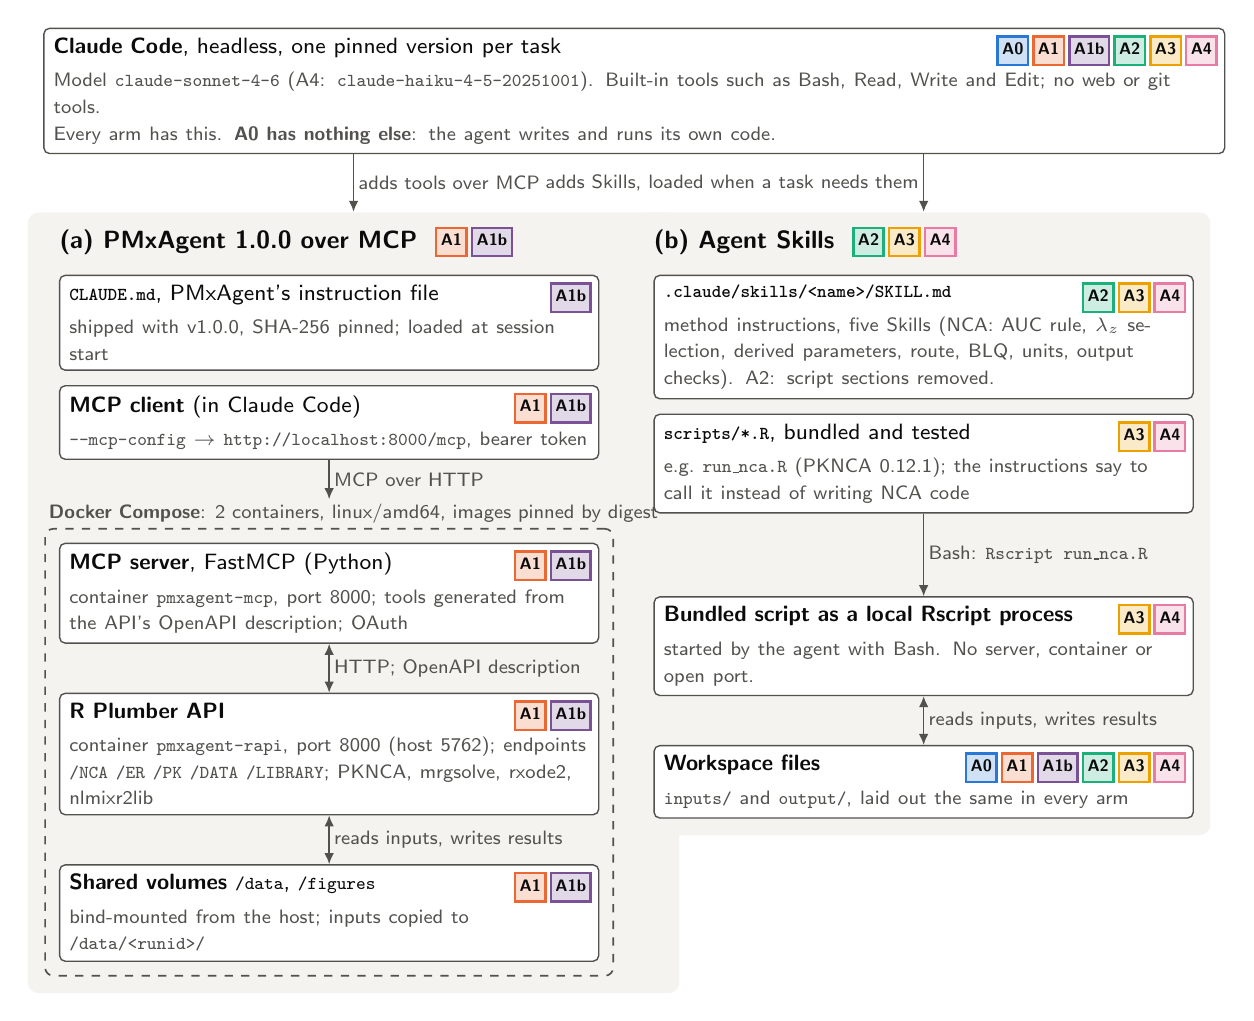
\begin{tikzpicture}

% ---- every arm: plain Claude Code ---------------------------------------------------------------------------------
\node[box=14.75cm, anchor=north west] (cc) at (0,0) {%
  \textbf{Claude Code}, headless, one pinned version per task\\[2.5pt]
  \detail{Model \code{claude-sonnet-4-6} (A4: \code{claude-haiku-4-5-20251001}). Built-in tools such as Bash, Read,
  Write and Edit; no web or git tools.}\\
  \detail{Every arm has this. \textbf{A0 has nothing else}: the agent writes and runs its own code.}};
\chips{cc}{\armchip{A0}\,\armchip{A1}\,\armchip{A1b}\,\armchip{A2}\,\armchip{A3}\,\armchip{A4}}

% ---- (a) PMxAgent: instructions (A1b only), MCP client, then the Docker stack ------------------------------------
\node[head] (ha) at ($(cc.south west)+(0.2,-0.95)$) {(a) PMxAgent 1.0.0 over MCP};
\headchips{ha}{\armchip{A1}\,\armchip{A1b}}

\node[box, anchor=north west] (cmd) at ($(ha.south west)+(0,-0.25)$) {%
  \textbf{\code{CLAUDE.md}}, PMxAgent's instruction file\\[2.5pt]
  \detail{shipped with v1.0.0, SHA-256 pinned; loaded at session start}};
\chips{cmd}{\armchip{A1b}}

\node[box, anchor=north west] (mcpc) at ($(cmd.south west)+(0,-0.18)$) {%
  \textbf{MCP client} (in Claude Code)\\[2.5pt]
  \detail{\code{-{}-mcp-config} $\rightarrow$ \code{http://localhost:8000/mcp}, bearer token}};
\chips{mcpc}{\armchip{A1}\,\armchip{A1b}}

\node[box, anchor=north west] (srv) at ($(mcpc.south west)+(0,-1.05)$) {%
  \textbf{MCP server}, FastMCP (Python)\\[2.5pt]
  \detail{container \code{pmxagent-mcp}, port 8000; tools generated from the API's OpenAPI description; OAuth}};
\chips{srv}{\armchip{A1}\,\armchip{A1b}}

\node[box, anchor=north west] (rapi) at ($(srv.south west)+(0,-0.62)$) {%
  \textbf{R Plumber API}\\[2.5pt]
  \detail{container \code{pmxagent-rapi}, port 8000 (host 5762); endpoints \code{/NCA /ER /PK /DATA /LIBRARY};
  PKNCA, mrgsolve, rxode2, nlmixr2lib}};
\chips{rapi}{\armchip{A1}\,\armchip{A1b}}

\node[box, anchor=north west] (vol) at ($(rapi.south west)+(0,-0.62)$) {%
  \textbf{Shared volumes} \code{/data}, \code{/figures}\\[2.5pt]
  \detail{bind-mounted from the host; inputs copied to \code{/data/<runid>/}}};
\chips{vol}{\armchip{A1}\,\armchip{A1b}}

\begin{scope}[on background layer]
  \node[dock, fit=(srv)(rapi)(vol)] (dock) {};
\end{scope}
\node[lab, anchor=south west] (docklab) at (dock.north west)
  {\textbf{Docker Compose}: 2 containers, linux/amd64, images pinned by digest};

\draw[flow] (mcpc.south) -- (docklab.north -| mcpc.south) node[lab, midway, right] {MCP over HTTP};
\draw[twoway] (srv.south) -- (rapi.north) node[lab, midway, right] {HTTP; OpenAPI description};
\draw[twoway] (rapi.south) -- (vol.north) node[lab, midway, right] {reads inputs, writes results};

% ---- (b) Agent Skills: instructions, bundled scripts, a local process, the workspace ------------------------------
\node[head] (hb) at ($(cc.south west)+(7.75,-0.95)$) {(b) Agent Skills};
\headchips{hb}{\armchip{A2}\,\armchip{A3}\,\armchip{A4}}

\node[box, anchor=north west] (skill) at ($(hb.south west)+(0,-0.25)$) {%
  \textbf{\code{.claude/skills/<name>/SKILL.md}}\\[2.5pt]
  \detail{method instructions, five Skills (NCA: AUC rule, $\lambda_z$ selection, derived parameters, route, BLQ,
  units, output checks). A2: script sections removed.}};
\chips{skill}{\armchip{A2}\,\armchip{A3}\,\armchip{A4}}

\node[box, anchor=north west] (scr) at ($(skill.south west)+(0,-0.18)$) {%
  \textbf{\code{scripts/*.R}}, bundled and tested\\[2.5pt]
  \detail{e.g.\ \code{run\_nca.R} (PKNCA 0.12.1); the instructions say to call it instead of writing NCA code}};
\chips{scr}{\armchip{A3}\,\armchip{A4}}

\node[box, anchor=north west] (rs) at ($(scr.south west)+(0,-1.05)$) {%
  \textbf{Bundled script as a local Rscript process}\\[2.5pt]
  \detail{started by the agent with Bash. No server, container or open port.}};
\chips{rs}{\armchip{A3}\,\armchip{A4}}

\node[box, anchor=north west] (ws) at ($(rs.south west)+(0,-0.62)$) {%
  \textbf{Workspace files}\\[2.5pt]
  \detail{\code{inputs/} and \code{output/}, laid out the same in every arm}};
\chips{ws}{\armchip{A0}\,\armchip{A1}\,\armchip{A1b}\,\armchip{A2}\,\armchip{A3}\,\armchip{A4}}

\draw[flow] (scr.south) -- (rs.north) node[lab, midway, right] {Bash: \code{Rscript run\_nca.R}};
\draw[twoway] (rs.south) -- (ws.north) node[lab, midway, right] {reads inputs, writes results};

% ---- panels and the step down from Claude Code -------------------------------------------------------------------
\begin{pgfonlayer}{panels}
  \node[fill=panel, rounded corners=4pt, inner sep=6pt, fit=(ha)(cmd)(mcpc)(docklab)(dock)] (pa) {};
  \node[fill=panel, rounded corners=4pt, inner sep=6pt, fit=(hb)(skill)(scr)(rs)(ws)] (pb) {};
\end{pgfonlayer}
\draw[flow] (cc.south -| pa.north) -- (pa.north) node[lab, midway, right] {adds tools over MCP};
\draw[flow] (cc.south -| pb.north) -- (pb.north) node[lab, midway, left] {adds Skills, loaded when a task needs them};

\end{tikzpicture}
\end{document}
